
\begin{frame} \frametitle{Le langage CQL}

Cassandra propose un langage, nommé CQL, inspiré de SQL, 
mais fortement restreint par l'absence de jointure. 

\vfill

CQL ne permet d'interroger qu'une seule table\,!

\vfill

De plus, d'autres types de restrictions s'appliquent\,! Elles s'expliquent toutes
par la volumétrie potentielle des tables.

\vfill

Nous allons étudier
tout cela.
\end{frame}



\begin{frame}[fragile] \frametitle{Premiers pas}

Sélectionnons tous les films.

\begin{minted}{sql}
select  * from movies;
\end{minted}

\vfill

Ou seulement les 20 premiers.
\begin{minted}{sql}
select  * from movies limit 20;
\end{minted}

\vfill
Retour en JSON
\begin{minted}{sql}
select JSON * from movies;
\end{minted}

\vfill
Accédons à un objet imbriqué.
\begin{minted}{sql}
select title, director.last_name from movies;
\end{minted}

\vfill
En revanche, on ne peut pas accéder aux éléments d'un ensemble.
\begin{minted}{sql}
select title, actors.last_name from movies;
\end{minted}
\end{frame}

\begin{frame}[fragile] \frametitle{La clause \texttt{where}}

Sélectionnons un film.

\begin{minted}{sql}
select  *  from movies where id='movie:33';
\end{minted}

Ou plusieurs

\begin{minted}{sql}
select  * from movies 
    where id in ('movie:33', 'movie:44214', 'movie:29845');
\end{minted}
 
Et si ce n'est pas la clé\,?

\begin{minted}{sql}
select  * from movies where title='Elle' ;
\end{minted}

\begin{verbatim}
Unable to execute CQL script. Cannot execute this query 
as it might involve data
filtering and thus may have unpredictable performance. 
\end{verbatim}

Essayons de comprendre.
\end{frame}

\begin{frame}[fragile] \frametitle{Structure d'un schéma}

\begin{columns}
    \begin{column}{0.45\textwidth}
  
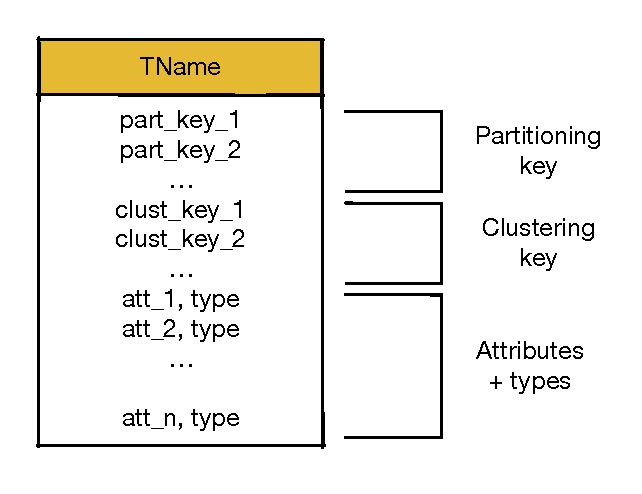
\includegraphics[height=.8\textwidth]{../figures/cassandra_chebotko.pdf}
  \end{column}
 \begin{column}{0.45\textwidth}
 \begin{minted}{sql}
 create table Tname (
   part_key_1 type,
   part_key_2 type,
   ... type,
   clust_key_1 type,
   ... type,
   att_1 type,
   att_2 type,
   ... type,
   primary key ( 
       (part_key_1, part_key2, ...), 
       (clust_key_1, clust_key_2, ...) 
       )
 )
 \end{minted}
\end{column}
\end{columns}

\end{frame}



\begin{frame}[fragile] \frametitle{Exemple\,: les rôles d'un film}

\begin{minted}{sql}
    create table Roles (
        id_film int,
        id_artiste int,
        role text,
        artist frozen<artist>,
        primary key (id_film, id_artiste)
     ) 
\end{minted}
\vfill

\begin{redbullet}
  \item La clé de partitionnement est  l'identifiant du film
  \item La
clé de regroupement est l'identifiant de l'artiste
\end{redbullet}
\end{frame}


\begin{frame}[fragile] \frametitle{Clé de partitionnement = placement}

\begin{columns}
    \begin{column}{0.45\textwidth}
  
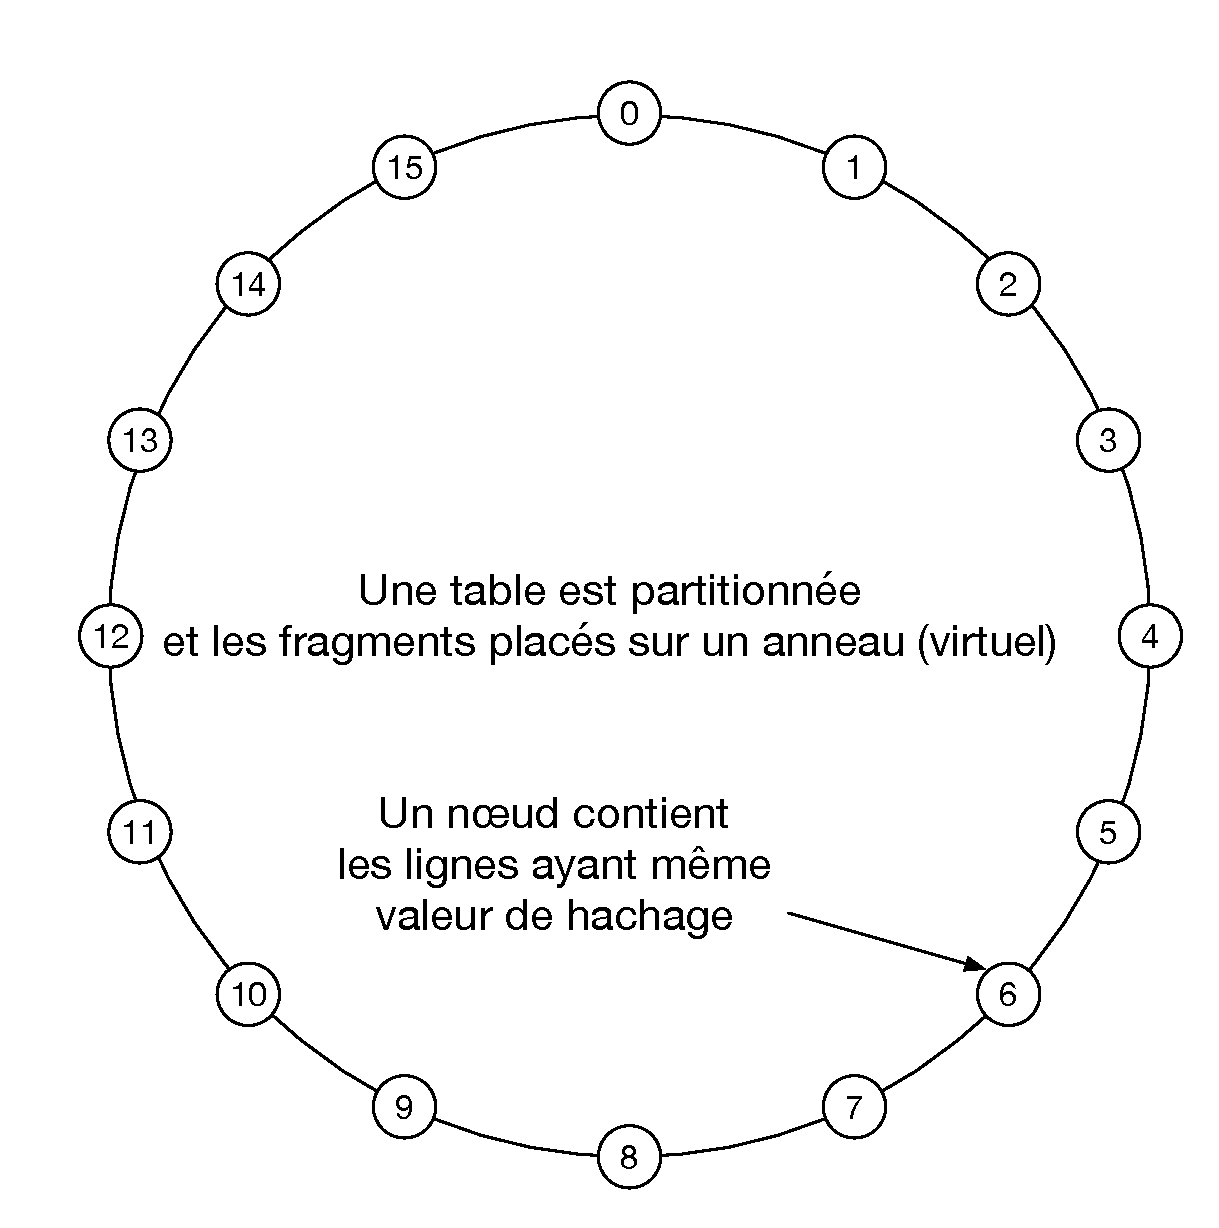
\includegraphics[height=\textwidth]{../figures/cassandra_anneau.pdf}
  \end{column}
 \begin{column}{0.45\textwidth}
\begin{redbullet}
		\item Pour chaque ligne on applique une fonction de hachage 
		          aux valeurs de la clé de \alert{partitionnement}
		\item La valeur de hachage détermine le placement dans le système distribué
		\item $\Rightarrow$ une requête incluant comme critère une clé de partitionnement
		     ne concerne qu'un seul serveur
	\end{redbullet}

\end{column}
\end{columns}

\end{frame}

%%%%%%%%%%
\begin{frame}[fragile] \frametitle{Clé de regroupement = contiguité}

\begin{columns}
    \begin{column}{0.45\textwidth}
    
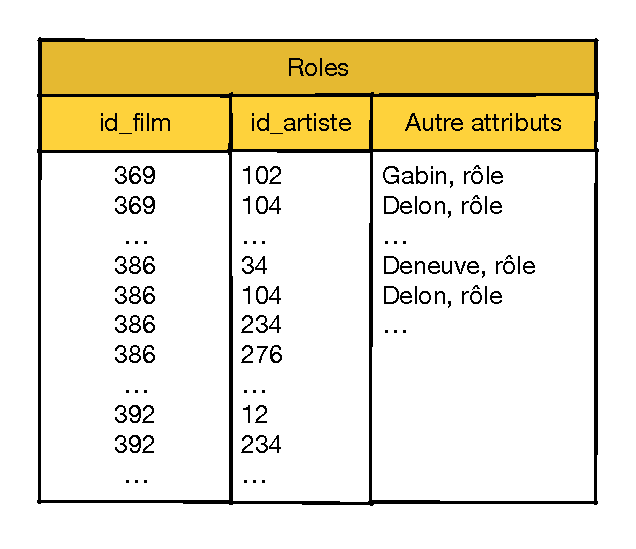
\includegraphics[height=\textwidth]{../figures/cassandra_clustering.pdf}
  
  \end{column}
 \begin{column}{0.45\textwidth}
\begin{redbullet}
		\item Dans un fragment (sur un serveur) les lignes sont triées 
		sur la clé primaire
		\item Pour une même valeur de partitionnement,  les lignes 
		   sont \alert{consécutives} et ordonnées sur la clé de regroupement
		\item $\Rightarrow$ une requête sur une préfixe de la clé 
		    primaire (part. + regroupement)
		     correspond à un parcours \alert{séquentiel} sur un seul nœud
	\end{redbullet}

\end{column}
\end{columns}

\end{frame}


%%%%%%%%%%
\begin{frame}[fragile] \frametitle{Restrictions sur les requêtes}

Toute recherche sur des critères autres qu'un préfixe de la clé entraîne un parcours
séquentiel

\vfill

Cassandra est conçu pour de très grandes bases de données, et le rejet 
de ces requêtes séquentielles est une précaution. 

\vfill

Principe: Cassandra limite les requêtes à celles dont le coût est proportionnel à la 
taille du résultat.

\vfill

On peut outrepasser avec la clause \texttt{allow filtering}.
\begin{minted}{sql}
select  * from movies 
     where country='US' and year=2020 allow filtering;
\end{minted}


\end{frame}
\end{document}